125. \begin{figure}[ht!]
\center{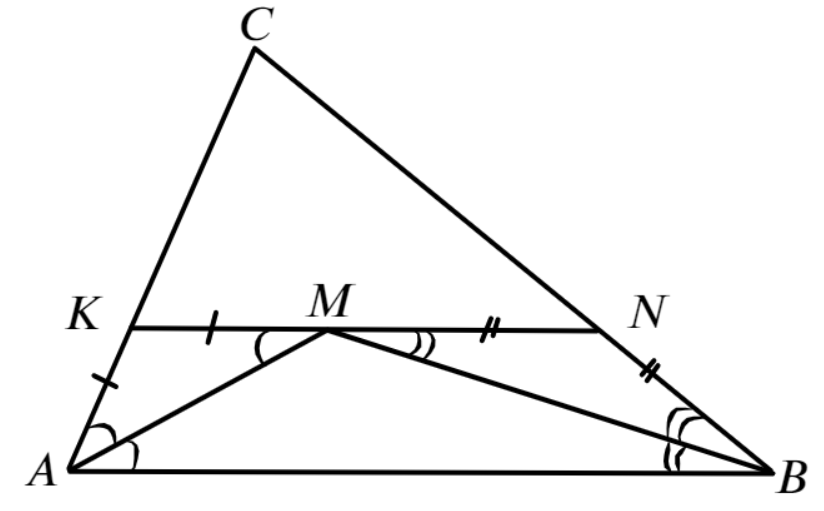
\includegraphics[scale=0.35]{g8-125.png}}
\end{figure}\\
Отметим равные углы, на которые делят угол биссектрисы и накрест лежащие: $\angle MAK=\angle MAB=\angle AMK$ и $\angle NBM=\angle MBA=\angle BMN.$ Тогда треугольники $AKM$ и $BNM$ являются равнобедренными и $AK=KM,\ BN=NM.$ Запишем разность $P_{\Delta ABC}-P_{\Delta KCN}=AB+AK+KC+CN+BN-CK-KM-NM-CN=AB=12-8=4.$\\
